\documentclass[tikz,border=3pt]{standalone}
\usepackage{amsmath,amssymb,bm}
\usetikzlibrary{arrows.meta,positioning,calc}
\definecolor{encblue}{HTML}{0072B2}
\definecolor{physgreen}{HTML}{007A59}
\begin{document}
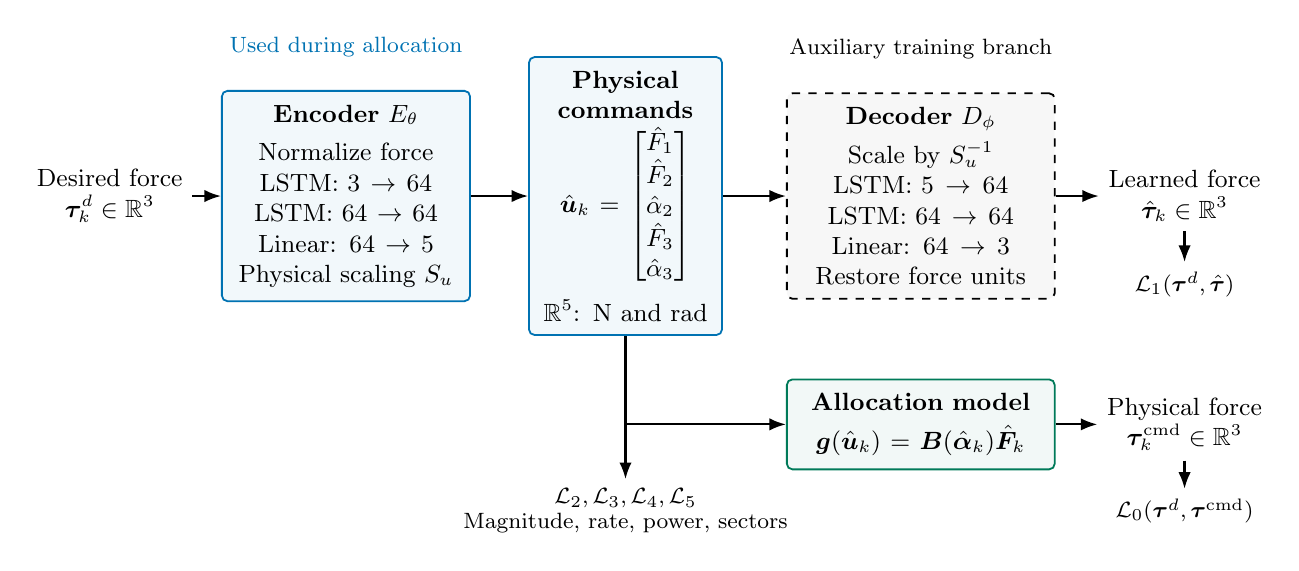
\begin{tikzpicture}[
  font=\fontsize{9}{11}\selectfont,
  block/.style={draw,rounded corners=2pt,align=center,inner sep=5pt,line width=.65pt},
  flow/.style={-{Latex[length=2.1mm]},line width=.8pt},
  loss/.style={align=center,font=\fontsize{8}{9}\selectfont}]
  \node[align=center] (request) at (0,0)
    {Desired force\\$\bm{\tau}^{d}_k\in\mathbb R^3$};
  \node[block,draw=encblue,fill=encblue!5,text width=2.8cm,minimum height=2.1cm] (encoder) at (3,0)
    {\textbf{Encoder $E_\theta$}\\[3pt]
     Normalize force\\
     LSTM: $3\rightarrow64$\\
     LSTM: $64\rightarrow64$\\
     Linear: $64\rightarrow5$\\
     Physical scaling $S_u$};
  \node[block,draw=encblue,fill=encblue!5,text width=2.1cm,minimum height=2.1cm] (command) at (6.55,0)
    {\textbf{Physical commands}\\[2pt]
     $\hat{\bm u}_k=\begin{bmatrix}\hat F_1\\\hat F_2\\\hat\alpha_2\\\hat F_3\\\hat\alpha_3\end{bmatrix}$\\[4pt]
     $\mathbb R^5$: N and rad};
  \node[block,dashed,fill=black!3,text width=3.05cm,minimum height=2.1cm] (decoder) at (10.3,0)
    {\textbf{Decoder $D_\phi$}\\[3pt]
     Scale by $S_u^{-1}$\\
     LSTM: $5\rightarrow64$\\
     LSTM: $64\rightarrow64$\\
     Linear: $64\rightarrow3$\\
     Restore force units};
  \node[align=center] (predicted) at (13.65,0)
    {Learned force\\$\hat{\bm\tau}_k\in\mathbb R^3$};
  \node[block,draw=physgreen,fill=physgreen!5,text width=3.05cm,minimum height=1.0cm] (physics) at (10.3,-2.9)
    {\textbf{Allocation model}\\[3pt]
     $\bm g(\hat{\bm u}_k)=\bm B(\hat{\bm\alpha}_k)\hat{\bm F}_k$};
  \node[align=center] (actual) at (13.65,-2.9)
    {Physical force\\$\bm\tau^{\rm cmd}_k\in\mathbb R^3$};
  \draw[flow] (request) -- (encoder);
  \draw[flow] (encoder) -- (command);
  \draw[flow] (command) -- (decoder);
  \draw[flow] (decoder) -- (predicted);
  \draw[flow] (command.south) |- (physics.west);
  \draw[flow] (physics) -- (actual);
  \node[loss] (constraints) at (6.55,-4.0)
    {$\mathcal L_2,\mathcal L_3,\mathcal L_4,\mathcal L_5$\\Magnitude, rate, power, sectors};
  \draw[flow] (command.south |- physics.west) -- (constraints.north);
  \node[loss] (reconstruction) at (13.65,-1.12)
    {$\mathcal L_1(\bm\tau^d,\hat{\bm\tau})$};
  \draw[flow] (predicted.south) -- (reconstruction.north);
  \node[loss] (ground) at (13.65,-4.0)
    {$\mathcal L_0(\bm\tau^d,\bm\tau^{\rm cmd})$};
  \draw[flow] (actual.south) -- (ground.north);
  \node[font=\fontsize{8}{9}\selectfont,text=encblue,above=3mm of encoder.north] {Used during allocation};
  \node[font=\fontsize{8}{9}\selectfont,above=3mm of decoder.north] {Auxiliary training branch};
\end{tikzpicture}
\end{document}
